\documentclass[12pt,a4paper]{report}
\parindent =0cm
\usepackage{amsmath}
\usepackage{amssymb,amsfonts, 
latexsym,cancel}
\usepackage{array}
\usepackage{bm}
\usepackage{float}
\usepackage{fancyhdr}
\usepackage{graphicx}
\usepackage{epstopdf}
\usepackage[colorlinks = true,
			linkcolor = black,
			citecolor = black,
			urlcolor = blue]{hyperref}
\usepackage{longtable}
\setcounter{MaxMatrixCols}{40}
\usepackage{multicol}
\usepackage{subfigure}
\usepackage{titling}
\usepackage{titlesec}
\usepackage{setspace}
\newcolumntype{E}{>{$}c<{$}}

\usepackage{anyfontsize}
\usepackage[utf8]{inputenc}
\usepackage{amsmath}
\usepackage{amsfonts}
\usepackage{amssymb}
\usepackage{makeidx}
\usepackage{graphicx}
%\usepackage{fourier}
\usepackage[left=2cm,right=2cm,top=2cm,bottom=2cm]{geometry}
\author{Guadalupe Monroy}
\begin{document}
\thispagestyle{empty} %% PARA QUITAR FORMATO DE PIES Y 
%\fbox{
\begin{minipage}[c][0.15\textheight][c]{0.17\textwidth}
    \begin{center}
        
\includegraphics[height=2.2cm, keepaspectratio=true]{imagenes/logocp} %% LOGO IZQUIERDO
    \end{center}
\end{minipage}
%}
%\fbox{
\begin{minipage}[c][0.15\textheight][t]{0.9\textwidth}
    \begin{center}
        {\scshape \Huge COLEGIO DE POSTGRADUADOS} %% NOMBRE DE LA UNIVERSIDAD
        \vspace{.5cm}   %% DEFINE EL ESPACIO ENTRE EL NOMBRE DE LA UNIVERSIDAD Y LA LÍNEA DOBLE
        \hrule height2.5pt  %% DEFINE EL ANCHO DE LA PRIMER LÍNEA
        \vspace{.1cm}    %% DEFINE EL ESPACIO ENTRE LAS DOS LINEAS
        \hrule height1pt  %% DEFINE EL ANCHO DE LA SEGUNDA LINEA (NORMALMENTE ES MAS DELGADA)
        \vspace{.4cm}   %% DEFINE EL ESPACIO ENTRE LA DOBLE LINEA Y EL NOMBRE DE LA DIVISIÓN
        {\scshape \LARGE  CAMPUS MONTECILLO}  %% NOMBRE DE LA DIVISIÓN
    \end{center}
\end{minipage}
%}

%\fbox{
\begin{minipage}[l][0.78\textheight][t]{0.1\textwidth}
    \begin{center}
    \hskip0pt
    \vrule width2.5pt height17cm    %% height definde la altura de la linea gruesa
        \hskip1mm
        \vrule width1pt height17cm  %% height define la altura de la linea delgada
        \end{center}
\end{minipage}
%}
%\fbox{
\begin{minipage}[c][0.78\textheight][t]{0.8\textwidth}
      \begin{center}
      \vspace{2cm}
        {\Large \scshape {PSEI-ESTADÍSTICA Y CIENCIA DE DATOS}}

        \vspace{2cm}

        \makebox[5cm][c]{\LARGE Examen. MODELOS LINEALES}  \\[16pt]
        PROFESOR DR. HUMBERTO VAQUERA HUERTA             \\[15pt]
        {\Large \textbf{{}}}\\[25pt]
        Al:\\[12pt]
        \textbf{ \Large {Guadalupe Monroy Hernández}}

        \vspace{2cm}
        
        \vspace{2.5cm}

        { Texcoco, Edo. México} \hskip2.5cm {}
      \end{center}
\end{minipage}
%}
\begin{enumerate}
\item Un diseño de bloques incompletos con $a$ tratamientos y $b$ bloques es similar a un diseño de bloques al azar completo, excepto que el tamaño de bloque $k$, es demasiado pequeño para permitir el juego completo de tratamientos pueda ser observado en cada bloque. En su lugar, $k < a$ tratamientos se da en cada bloque. Un diseño de bloques incompletos balanceados (BIBD) es un diseño de bloques incompletos con la propiedad de que cada par de tratamientos se presenta junto (es decir, juntos en el mismo bloque) el mismo número de veces. Una buena característica de un BIBD es que todas las diferencias por pares entre los efectos del tratamiento son estimadas con la misma precisión. (Este diseño se usa mucho en experimentos de Genética Vegetal). Considere el siguiente BIBD:\\

\begin{tabular}{| c | c | c |}
\hline
1 & 2 & 3\\ \hline
A \textit{y11} & A \textit{y12} & B \textit{y23}\\
B \textit{y21} & C \textit{y23} & C \textit{y33}\\
\hline
\end{tabular}
\\

Donde, $Y_{ij}$ denota una respuesta del el i-esimo tratamiento en el j-esimo bloque, y A, B, C Denotan los a = 3 tratamientos en el experimento. Note que los datos son $\lbrace Y_{ij}\rbrace$, $i = 1, 2, 3, j = 1, 2, 3$ pero solo hay $n = 6$ observaciones presentes, por lo que no todas las combinaciones de $i$ y $j$ son  observadas. Note que el tamaño de bloque es $k = 2$ el cual es muy pequeño para poner todos los $a = 3$ tratamientos. Sin embargo, es un bloque incompleto balanceado porque todos los pares posibles ((A, B),(A, C),(B, C)) ocurren el mismo número de veces (una).\\

Modelo usual para este diseño es:\\
$$y_{ij}=\mu +\alpha_{i}+\beta_{j}+\epsilon_{ij},\quad \lbrace\epsilon_{ij}\rbrace iid\sim N(0,\sigma^{2}) $$

\begin{itemize}
\item Escriba el modelo en notación Matricial $Y = X\beta + \epsilon$. Es decir, indique de manera explícita la Matriz diseño X y el resto de componentes del modelo.\\

\begin{equation*}
\begin{bmatrix}
y_{11}\\
y_{12}\\
y_{21}\\
y_{23}\\
y_{32}\\
y_{33}\\
\end{bmatrix}
=\begin{bmatrix}
1 & 1 & 0 & 0 & 1 & 0 & 0 \\
1 & 1 & 0 & 0 & 0 & 1 & 0 \\
1 & 0 & 1 & 0 & 1 & 0 & 0 \\
1 & 0 & 1 & 0 & 0 & 0 & 1 \\
1 & 0 & 0 & 1 & 0 & 1 & 0 \\
1 & 0 & 0 & 1 & 0 & 0 & 1 \\
\end{bmatrix}
\begin{bmatrix}
\mu\\
\alpha_{1}\\
\alpha_{2}\\
\alpha_{3}\\
\beta_{1}\\
\beta_{2}\\
\beta_{3}\\
\end{bmatrix}+
\begin{bmatrix}
\epsilon_{11}\\
\epsilon_{12}\\
\epsilon_{21}\\
\epsilon_{23}\\
\epsilon_{32}\\
\epsilon_{33}\\
\end{bmatrix}
\end{equation*}

La matriz diseño tiene una columna de 1 para la media, tres columnas para los tratamientos y tres
columnas para los bloques.

\end{itemize}

%-----EJERCIO 2-----------
\item La función de producción CES (elasticidad sustitución constante) que relaciona la producción $Y$ con el trabajo $X1$ y el capital $X2$ está dada por:\\

$$ Y=A\lbrace \alpha X^{\beta}_{1}+(1-\alpha)X^{\beta}_{2}\rbrace^{\dfrac{\gamma}{\beta}} + \epsilon$$


donde: $-\beta \leq 1$ es el parámetro de sustitución $\gamma > 0$ es el parámetro que determina el grado de homogeneidad de la función. $\alpha \in \left[ 0, 1\right[$ y $\left( 1 - \alpha\right( $ son parámetros que representan las preferencias relativas que el individuo tiene por los bienes. ( casos especiales $\beta = 0$ es la función Cobb Douglas, con $\beta=-\infty$ Complementos Perfectos, con $\beta = 0$ substitutos Perfectos).

\begin{enumerate}
\item ¿Es un modelo lineal o no lineal? (justifique su respuesta).\\

No es un modelo lineal. Exponenciación compuesta: El término $\lbrace \alpha X^{\beta}_{1}+(1-\alpha)X^{\beta}_{2}\rbrace$ esta elevado a la ${\dfrac{\gamma}{\beta}}$. Esta exponenciación crea una relación no lineal entre la producción Y y los factores de producción X1 y X2. Incluso si $\beta$ fuera 1, la relación seguiría siendo no lineal debido a la potencia ${\dfrac{\gamma}{\beta}}$.\\

Tamnién se puede ver al derivar la función $Y$ con respecto a $\beta$.\\
Usamos la formula $\dfrac{d}{dx}a^{u}=a^{u}ln a\dfrac{d}{dx}u$

\begin{align*}
\dfrac{\partial}{\partial\beta}Y&=\dfrac{\partial}{\partial\beta}A\lbrace \alpha X^{\beta}_{1}+(1-\alpha)X^{\beta}_{2}\rbrace^{\dfrac{\gamma}{\beta}}\\
&=A\lbrace \alpha X^{\beta}_{1}+(1-\alpha)X^{\beta}_{2}\rbrace^{\dfrac{\gamma}{\beta}}ln\left(\lbrace \alpha X^{\beta}_{1}+(1-\alpha)X^{\beta}_{2}\rbrace \right)\dfrac{\partial}{\partial\beta}\left(\dfrac{\gamma}{\beta}\right)
\end{align*}
La derivada parcial de $Y$ en función de $\beta$ no es independiente del parámetro. No es una función lineal.

\item Considerando el modelo sin el termino de error, es posible transformar a una función lineal( es
linealizable?).\\
Usando una transformación logarítmica.\\

$$ Y=A\lbrace \alpha X^{\beta}_{1}+(1-\alpha)X^{\beta}_{2}\rbrace^{\dfrac{\gamma}{\beta}} + \epsilon\rightarrow ln(Y)=ln(A)+{\dfrac{\gamma}{\beta}}*ln(\lbrace \alpha X^{\beta}_{1}+(1-\alpha)X^{\beta}_{2}\rbrace)$$
Sin embargo, es importante tener en cuenta que esta transformación no es exacta. Ya no es posible trasnformar a una función lineal a $Y$.\\

\item El caso $\beta = 0$ es la función Cobb Douglas porque es considerado linelizable?\\

La función de producción Cobb-Douglas es una función lineal porque la relación entre la producción y los factores de producción es una relación lineal. En particular, la relación entre la producción y el trabajo es una relación lineal, ya que la función de producción Cobb-Douglas implica una relación de multiplicación entre la producción y el trabajo.\\
Es posible transformar a una función lineal, $Y(X_{1},X_{2})=AX_{1}^{\beta}X_{2}^{\alpha}$\\
\begin{align*}
ln\left( Y(X_{1},X_{2})\right)&=ln\left(AX_{1}^{\beta}X_{2}^{\alpha}\right)\\
&=lnA + \beta ln X_{1}+\alpha ln X_{2}
\end{align*}
Los parámetros están en forma lineal. Las derivadas parciales de la transformación resultan en que el modelo es lineal bajo la transformación logarítmica.\\

\end{enumerate}

%--------EJERCICIO 3-------

\item Escriba el modelo en notación matricial:\\
\begin{enumerate}
\item Modelo ANOVA dos vias de clasificación con interacción:\\

$$y_{ijk}=\mu +\alpha_{i}+\beta_{i}+\phi_{ji}+\varepsilon_{ijk}, i=1,2;j=1,2,k=1,2$$

\begin{equation*}
\begin{bmatrix}
y_{111}\\
y_{121}\\
y_{211}\\
y_{221}\\
y_{112}\\
y_{122}\\
y_{212}\\
y_{222}\\
\end{bmatrix}
=\begin{bmatrix}
1 & 1 &0& 1& 0& 1& 0& 0& 0\\
1 &1& 0& 0& 1& 0& 1& 0& 0\\
1& 0& 1& 1& 0& 0& 0& 1& 0\\
1& 0& 1& 0& 1& 0& 0& 0& 1\\
1& 1& 0& 1& 0& 1& 0& 0& 0\\
1& 1& 0& 0& 1& 0& 1& 0& 0\\
1& 0& 1& 1& 0& 0& 0& 1& 0\\
1& 0& 1& 0& 1& 0& 0& 0& 1\\
\end{bmatrix}
\begin{bmatrix}
\mu\\
\alpha_{1}\\
\alpha_{2}\\
\beta_{1}\\
\beta_{2}\\
\phi_{11}\\
\phi_{12}\\
\phi_{21}\\
\phi_{22}
\end{bmatrix}+
\begin{bmatrix}
\epsilon_{111}\\
\epsilon_{121}\\
\epsilon_{211}\\
\epsilon_{221}\\
\epsilon_{112}\\
\epsilon_{122}\\
\epsilon_{212}\\
\epsilon_{222}\\
\end{bmatrix}
\end{equation*}
Los factores, sean A y B, solo tienen dos tratamientos, por lo que se tienen cuatro interacciones posibles entre los niveles de A y B.



\end{enumerate}
%-----EJERCICIO 4--------------
\item \textbf{Modelos de curva de crecimiento de Richards}\\
El modelo de curva de crecimiento Gompertz. La curva se adaptó en epidemiología para la predicción en
tiempo real de brotes de enfermedades; los ejemplos incluyen el brote de COVID-19.\\
$$ Y(t)=ae^{-e^{-b(t-c)}}+\varepsilon_{t} $$

¿Dónde $Y (t)$ está el número de muertes acumuladas por cada día? $a$ es el número máximo de muertes
acumuladas al final de la epidemia; $b$ es la tasa de crecimiento relativo estimada del total de muertes; $t$ es el número de días desde el primer caso y $c$ es el momento en el que se estima el punto de inflexión de la curva.\\

\begin{enumerate}
\item ¿Es un modelo lineal o no lineal? (justifique su respuesta).\\

Tomamos las derivadas parciales de $Y(t)$ con respecto a los parametros para saber si el modelo es lineal.\\

\begin{align*}
\dfrac{\partial}{\partial a}Y(t)&=\dfrac{\partial}{\partial a}\left[ae^{-e^{-b(t-c)}}\right]\\
&=e^{-e^{-b(t-c)}}\\
\dfrac{\partial}{\partial b}Y(t)&=\dfrac{\partial}{\partial a}\left[ae^{-e^{-b(t-c)}}\right]\\
&=\left[ae^{-e^{-b(t-c)}}\right]\dfrac{\partial}{\partial b}-e^{-b(t-c)}
\end{align*}

La derivada parcial es independiente del parametro $a$, sin embargo para el caso del parametro $b$, es evidente que este resulta no ser independiente. Con esto podemos concluir que no es un modelo lineal.


\item Considerando el modelo sin el termino de error, es posible transformar a una función lineal( es
linealizable?).\\

Aplicando logaritmo natural, se intentará transformar a un modelo lineal.\\


\begin{align*}
ln(Y(t))&=ln\left( ae^{-e^{-b(t-c)}}\right)\\
&=ln(a)+ ln\left(e^{-e^{-b(t-c)}}\right)\\
&=ln(a)-e^{-b(t-c)}
\end{align*}
Hasta este punto no es posible transformar a una funcion lineal, por lo que no es linealizable.

\item Grafique suponiendo $Y (t) = 98008.0988e^{-e^{-0.01830109(t-117.8062)}}+\varepsilon_{t} $ esto encontraron: Conde-Gutiérrez, R.A., Colorado, D. y Hernández-Bautista, S.L. Comparison of an artificial neural network and Gompertz model for predicting the dynamics of deaths from COVID-19 in México. Nonlinear Dyn 104, 4655–4669 (2021).\\
https://doi.org/10.1007/s11071-021-06471-7.\\
que opinión le merece esto, le parece que solo murieron 98008 mexicanos? A veces no es solo publicar por publicar.

\begin{verbatim}
library(ggplot2)
y<-function(t){98008.0988*exp(-exp(- 0.01830109*(t-117.8062)))
  }
t <-c(1:365)

plot(y(t),col='red',type = 'l',xlab = 'Número de días desde el primer caso', 
     ylab = 'Número de muertes acumuladas por día')

\end{verbatim}
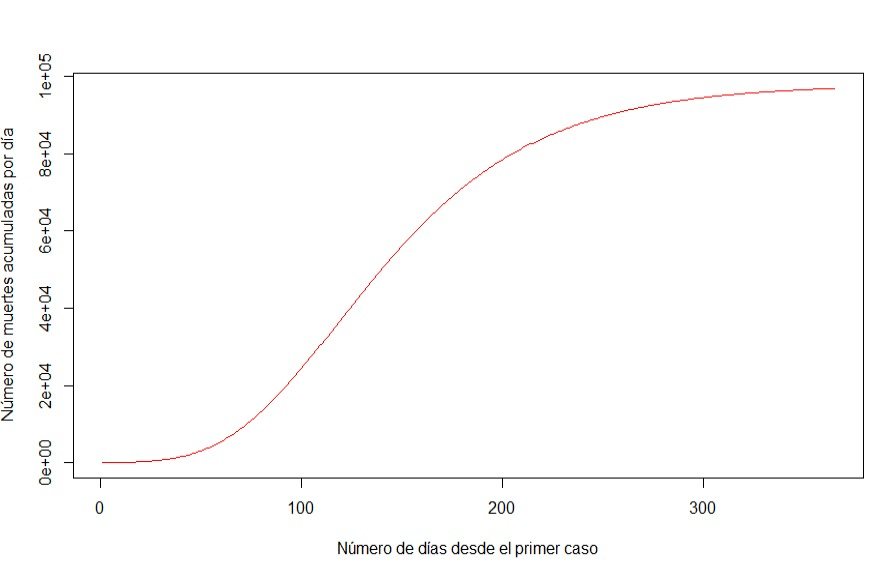
\includegraphics[height=8cm, keepaspectratio=true]{imagenes/grap}\\

La estimación del número de muertes es por mucho, muy alejada a lo que realmente acontecio. 
\end{enumerate}

%----EJERCICIO 5--------------
\item Se realizó un experimento para evaluar los efectos de tres nuevos alimentos ricos en nutrientes (F) para producir un aumento de peso acelerado en conejillos de indias. Se administraron los alimentos a animales de tres cepas ( S ) y se registraron sus ganancias de peso ( $y$ ) en gramos. Como es común en estudios de este tipo, los pesos iniciales de ( $x$ ) de los animales también se registraron para su uso como covariable. Los datos son:\\


\begin{tabular}{| c | c  c | c  c | c  c |}
\hline
\multicolumn{3}{ |c| }{Alimento A}&& \multicolumn{1}{ |c| }{Alimento B} && \multicolumn{1}{ |c| }{Alimento C}\\ \hline
Cepa & x & y & x & y & x & y \\ \hline
1& 152 &301 &160 &298 &162 &336\\
2 &177 &337 &168 &310 &181 &379\\
3 &114 &241 &125 &234 &122 &258\\
\hline
\end{tabular}

Considere el modelo de análisis de covarianza con dos factores de estudio:\\
$$y_{ij}=\mu +\alpha_{i}+\beta_{j}+\gamma x_{ij}+\varepsilon_{ij}, \varepsilon_{ij}\sim N(0,\sigma^2)$$

$\alpha_i$ =efecto del alimento $i$, $\beta_j$ =efecto de la cepa $j$.\\
Escriba el modelo en forma matricial $y = X\beta + \varepsilon$, especifique los componentes.\\

\begin{equation*}
\begin{bmatrix}
301\\
337\\
241\\
298\\
310\\
234\\
336\\
379\\
258\\
\end{bmatrix}
=\begin{bmatrix}
1 &1& 0& 0& 1& 0& 0& 152\\
1 &1& 0& 0& 0& 1& 0& 177\\
1& 1& 0& 0& 0& 0& 1& 114\\
1& 0& 1& 0& 1& 0& 0& 160\\
1& 0& 1& 0& 0& 1& 0& 168\\
1& 0& 1& 0& 0& 0& 1& 125\\
1& 0& 0& 1& 1& 0& 0& 162\\
1& 0& 0& 1& 0& 1& 0& 181\\
1& 0& 0& 1& 0& 0& 1& 122\\
\end{bmatrix}
\begin{bmatrix}
\mu\\
\alpha_{1}\\
\alpha_{2}\\
\alpha_{3}\\
\beta_{1}\\
\beta_{2}\\
\beta_{3}\\
\gamma
\end{bmatrix}+
\begin{bmatrix}
\epsilon_{11}\\
\epsilon_{12}\\
\epsilon_{13}\\
\epsilon_{21}\\
\epsilon_{22}\\
\epsilon_{23}\\
\epsilon_{31}\\
\epsilon_{32}\\
\epsilon_{33}\\
\end{bmatrix}
\end{equation*}




%--------------EJERCICIO 6-------------------------

\item Considere el modelo de Superficie de Respuesta:
$$y = \beta_{0} + \beta_{1} x_{1} + \beta_{2} x_{2} + \beta_{12} x_{1}x_{2} + \beta_{11} x_{21} + \beta_{22} x_{22} + \varepsilon; \varepsilon \sim N(0, \sigma^2)$$

\begin{tabular}{| c | c | c |}
\hline
x1 & x2 & y\\ \hline
30 &150 &39.3\\
40 &150 &40.9\\
30 &160 &40\\
40 &160 &41.5\\
35 &155 &40.3\\
35 &155 &40.5\\
35 &155 &40.7\\
35 &155 &40.2\\
35 &155 &40.6\\
\hline
\end{tabular}

\begin{enumerate}
\item ¿Es un modelo lineal o no lineal? (justifique su respuesta).\\

Para saber si es un  modelo lineal obtenemos las derivadas parciale de cada parametro.\\
$$\dfrac{\partial}{\partial\beta_{1}}y=\dfrac{\partial}{\partial\beta_{1}}\left(\beta_{0} + \beta_{1} x_{1} + \beta_{2} x_{2} + \beta_{12} x_{1}x_{2} + \beta_{11} x_{1}^{2} + \beta_{22} x_{2}^{2} + \varepsilon\right)=x_{1}$$

$$\dfrac{\partial}{\partial\beta_{2}}y=\dfrac{\partial}{\partial\beta_{1}}\left(\beta_{0} + \beta_{1} x_{1} + \beta_{2} x_{2} + \beta_{12} x_{1}x_{2} + \beta_{11} x_{1}^{2} + \beta_{22} x_{2}^{2} + \varepsilon\right)=x_{2}$$

$$\dfrac{\partial}{\partial\beta_{12}}y=\dfrac{\partial}{\partial\beta_{1}}\left(\beta_{0} + \beta_{1} x_{1} + \beta_{2} x_{2} + \beta_{12} x_{1}x_{2} + \beta_{11} x_{1}^{2} + \beta_{22} x_{2}^{2} + \varepsilon\right)=x_{1}x_{2}$$

$$\dfrac{\partial}{\partial\beta_{11}}y=\dfrac{\partial}{\partial\beta_{1}}\left(\beta_{0} + \beta_{1} x_{1} + \beta_{2} x_{2} + \beta_{12} x_{1}x_{2} + \beta_{11} x_{1}^{2} + \beta_{22} x_{2}^{2} + \varepsilon\right)=x_{1}^{2}$$

$$\dfrac{\partial}{\partial\beta_{22}}y=\dfrac{\partial}{\partial\beta_{1}}\left(\beta_{0} + \beta_{1} x_{1} + \beta_{2} x_{2} + \beta_{12} x_{1}x_{2} + \beta_{11} x_{1}^{2} + \beta_{22} x_{2}^{2} + \varepsilon\right)=x_{2}^{2}$$

Dado que las derivadas son independientes de los parametros se puede concluir que es un modelo lineal.\\

\item ¿Cuál es su matriz diseño?

\begin{equation*}
\textbf{X}=\begin{bmatrix}
1 & x_{11}& x_{12} & x_{11}x_{12} & x_{11}^{2} & x_{12}^{2}\\
1 & x_{21}& x_{22} & x_{21}x_{22} & x_{21}^{2} & x_{22}^{2}\\
1 & x_{31}& x_{32} & x_{31}x_{32} & x_{31}^{2} & x_{32}^{2}\\
1 & x_{41}& x_{42} & x_{41}x_{42} & x_{41}^{2} & x_{42}^{2}\\
1 & x_{51}& x_{52} & x_{51}x_{52} & x_{51}^{2} & x_{52}^{2}\\
1 & x_{61}& x_{62} & x_{61}x_{62} & x_{61}^{2} & x_{62}^{2}\\
1 & x_{71}& x_{72} & x_{71}x_{72} & x_{71}^{2} & x_{72}^{2}\\
1 & x_{81}& x_{82} & x_{81}x_{82} & x_{81}^{2} & x_{82}^{2}\\
1 & x_{91}& x_{92} & x_{91}x_{92} & x_{91}^{2} & x_{92}^{2}
\end{bmatrix}
\end{equation*}
\begin{equation*}
\textbf{X}=\begin{bmatrix}
1 & 30 & 150 & 4500 & 900 & 22500\\
1 & 40 & 150 & 6000 & 1600 & 22500\\
1 & 30 & 160 & 4800 & 900 & 22600\\
1 & 40 & 160 & 6400 & 1600 & 25600\\
1 & 35 & 155 & 5425 & 1225 & 24025\\
1 & 35 & 155 & 5425 & 1225 & 24025\\
1 & 35 & 155 & 5425 & 1225 & 24025\\
1 & 35 & 155 & 5425 & 1225 & 24025\\
1 & 35 & 155 & 5425 & 1225 & 24025\\
\end{bmatrix}
\end{equation*}
\end{enumerate}

\end{enumerate}
\end{document}